\documentclass[8pt]{beamer}
\usepackage{amsmath}
\usepackage{amssymb}
\usepackage{graphicx}
\usepackage{hyperref}
\usepackage{color}
\usepackage{float}
\usepackage{subfig}


%\usepackage{sidecap}
\title{Random loops model can explain the appearance of Topologically Associating Domains (TADs)}
\author{Ofir Shukron}
\usetheme{Madrid}
\usecolortheme{dolphin}

\begin{document}

\begin{frame} %{Stochastic Simulation of Topologically Associating Domains}
\titlepage
\end{frame}

\section{Introduction}\label{section_introduction}
\begin{frame}{Introduction}
\begin{enumerate}
\item The spatio-temporal organization of the chromatin has significant implication of  cellular activities, such as gene expression and regulation. 
\item however, the spatial organization of the chromatin is not entirely known.
\item DNA looping has shown to be a mechanism for long range gene regulation.
\item here we show that using  random polymer looping model and fitting it to the  experimental chromatin looping data we can explain the appearance of conserved structures in chromatin called TADs.
\end{enumerate}
\end{frame}


\begin{frame}{Agenda}
\tableofcontents
\end{frame}


\section{The experimental setting}\label{section_theExperimentalSetting}
\subsection{Chromosome Conformation Capture Experiments}\label{subsection_chromosomeConformationCaptureExperiments}
\begin{frame}{Chromosome Conformation Capture Experiments}
A set of methods to simultaneously record millions of looping events occurring within the genome (specific or unspecific). 

The general steps are:
\begin{enumerate}
\item intact nuclei are extracted from millions of cells 
\item Formaldehyde induces protein-DNA and protein-protein cross-links
\item restriction enzymes digest the cross-linked DNA
\item cross-linked DNA is purified, diluted and ligated
\item cross-links are reversed
\item PCR to amplify ligation junctions
\item histogram of segment encounter is produced
\end{enumerate}
\begin{figure}[H]
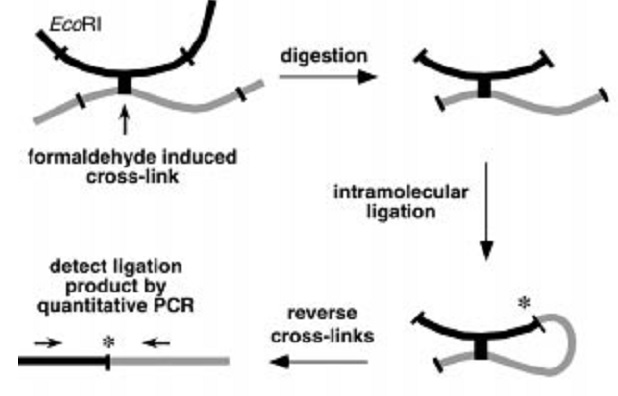
\includegraphics[scale=0.3]{3Cschematic}
\end{figure}
\end{frame}

\subsection{The experimental Data}\label{subsection_theExperimentalData}
\begin{frame}{The experimental data}
\begin{itemize}
\item Two replicate of the CC experiments were conducted by Nora et. al 2012. 
\item we focus on a 920,432 bp subset of the data, around the X inactivation center of the X chromosome in mouse embryonic stem cells. 
\item the region harbors the Xist enhancer and Tisx promoter.
\item we have the segments' encounter frequencies from the two experimental replicates.
\end{itemize}
\end{frame}

\begin{frame}{Topologically Associating Domains (TADs)}
Conserved structures of chromosome interactions on the Mb scale, with higher inter than intra-segment interactions
It is believed that the TAD forms a 'regulatory unit' for regulating gene expression, as can be seen by the correlation of gene expression located on the same TAD
\centering
\begin{figure}[H]

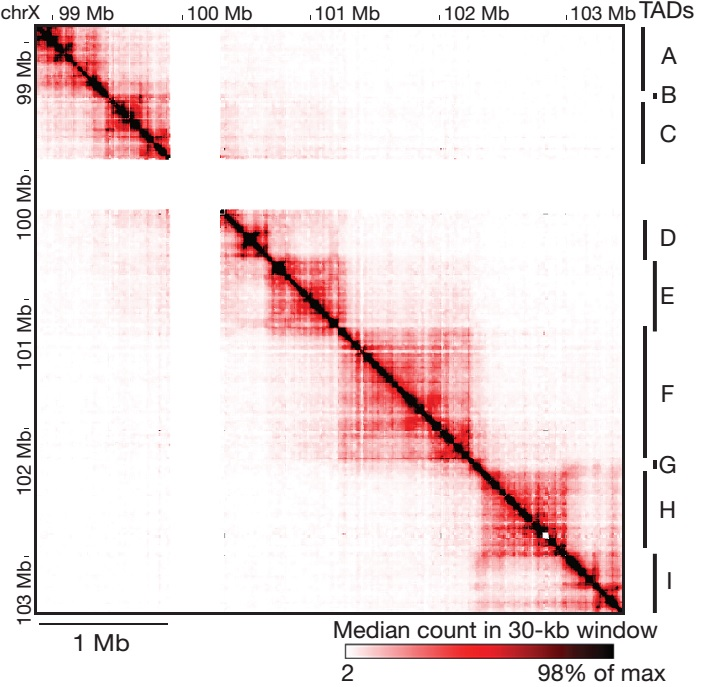
\includegraphics[scale=0.2]{TADsOfTheXChromosome_NoraEtAl2012}
\quad
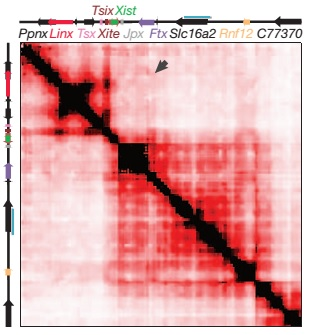
\includegraphics[scale=0.25]{TadDandENoraEtAl2012} 
\quad
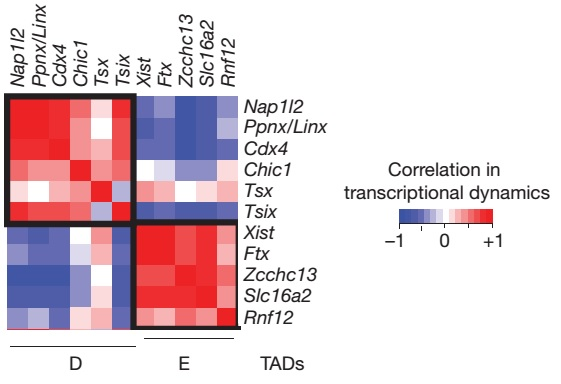
\includegraphics[scale=0.27]{transcriptionCorrelationTadDandENoraEtAl2012}
\caption{\tiny{The 4.5 Mb region (left), enlargement of TAD D and E (center). Displayed median count in a 30kb window every 6kb, gene expression correlation (right)}}
\label{fig:TADsOfTheXChromosome_NoraEtAl2012}
\end{figure}
\end{frame}

\section{Analysis of the data}\label{section_analysisOfTheData}
\begin{frame}{From restriction segments to beads}
\begin{itemize}
\item To coarse-grain the data, we choose a bead-size of 3000 bp, corresponding to the mean segment length resulted from the digestion of EcoRIII enzyme. 

\begin{figure}[H]
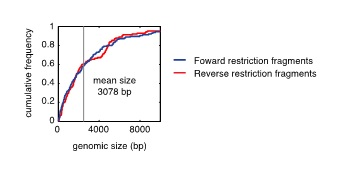
\includegraphics[scale=0.55]{restrictionSegmentLengthDistributionLucaetal}
\end{figure}
\item the genomic section was evenly partitioned by 3000 bp beads. Each segment receives a start and end index according to the beads it covers. 
\item for example, 
\begin{tabular}[H]{|l| l| l|}
\hline
bp range & start ind & end ind\\
\hline
500-3500   & 1         & 2 \\
4000-4500  & 2         & 2 \\   
5000-12001 & 2         & 4 \\       
\hline  
\end{tabular}
\end{itemize}
\end{frame}


\subsection{TAD D and E}\label{subsection_tadDAndE}
\begin{frame}{Bead encounter frequecy}
\framesubtitle{TAD D and E}
\begin{itemize}
\item We work with the average of the two experimental replicates
\item a total length of 920,432 bp - resulting in 307 beads (TAD D 107 beads, TAD E 200 beads)
\item We calculate the 'one-sided' encounter probability vs. distance (bead units) for each bead
\item the mean encounter probability difference, shows that the data is left-right symmetric

\begin{figure}[H]
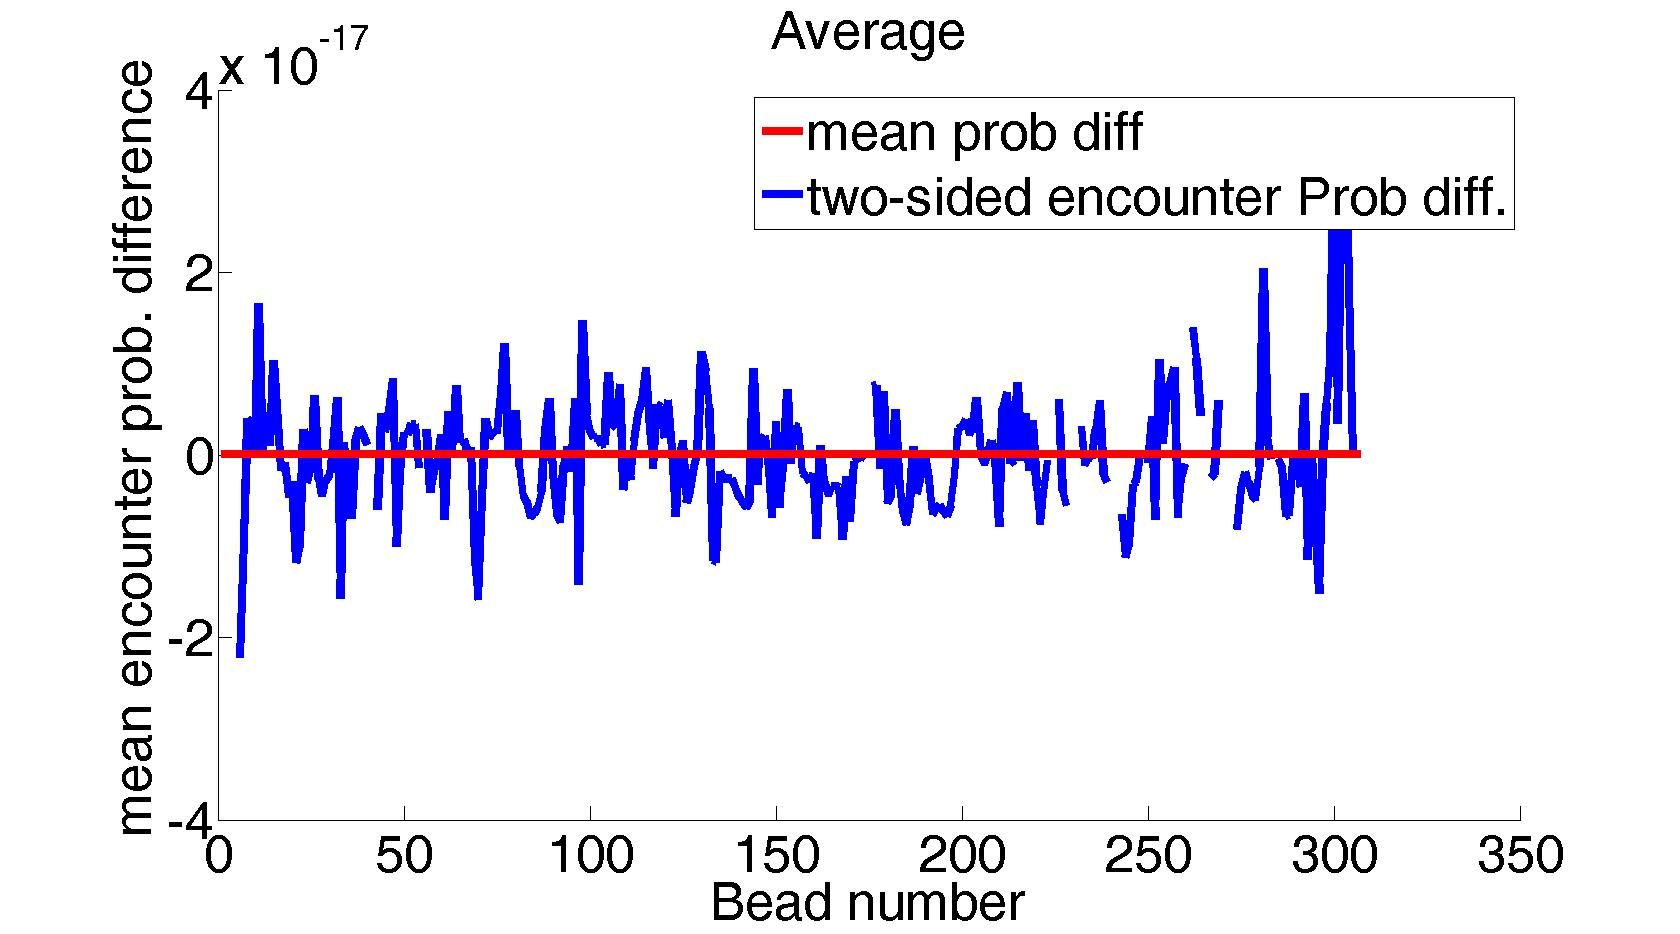
\includegraphics[scale=0.05]{symmetryOfTheEncounterProbability307BeadsAverage}
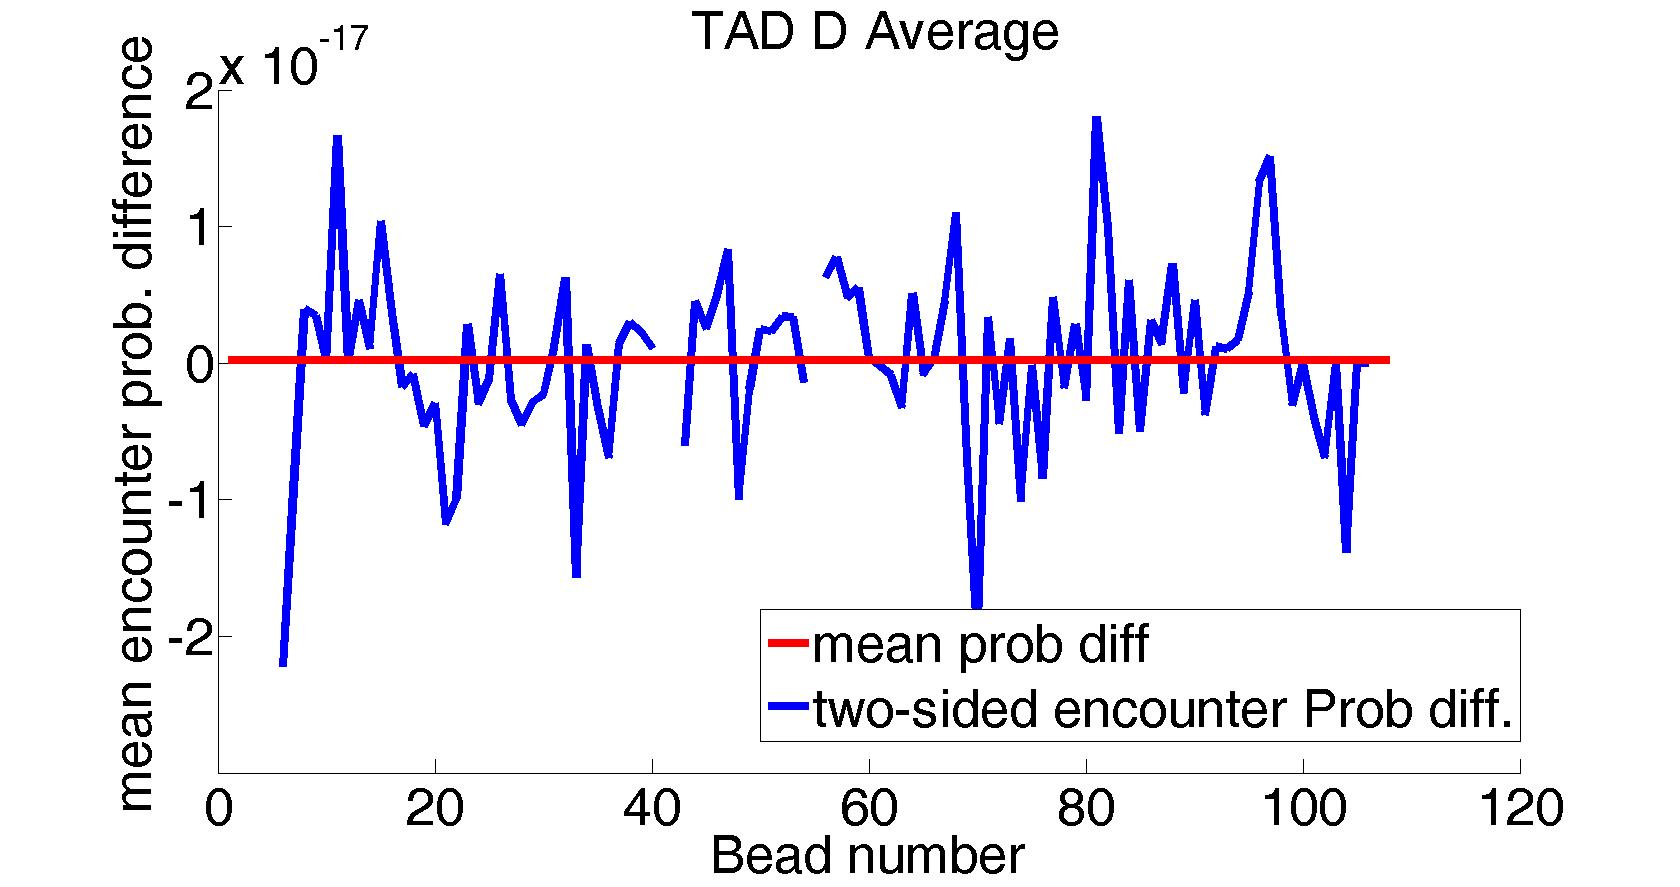
\includegraphics[scale=0.05]{symmetryOfTheEncounterProbabilityTADDAverage}
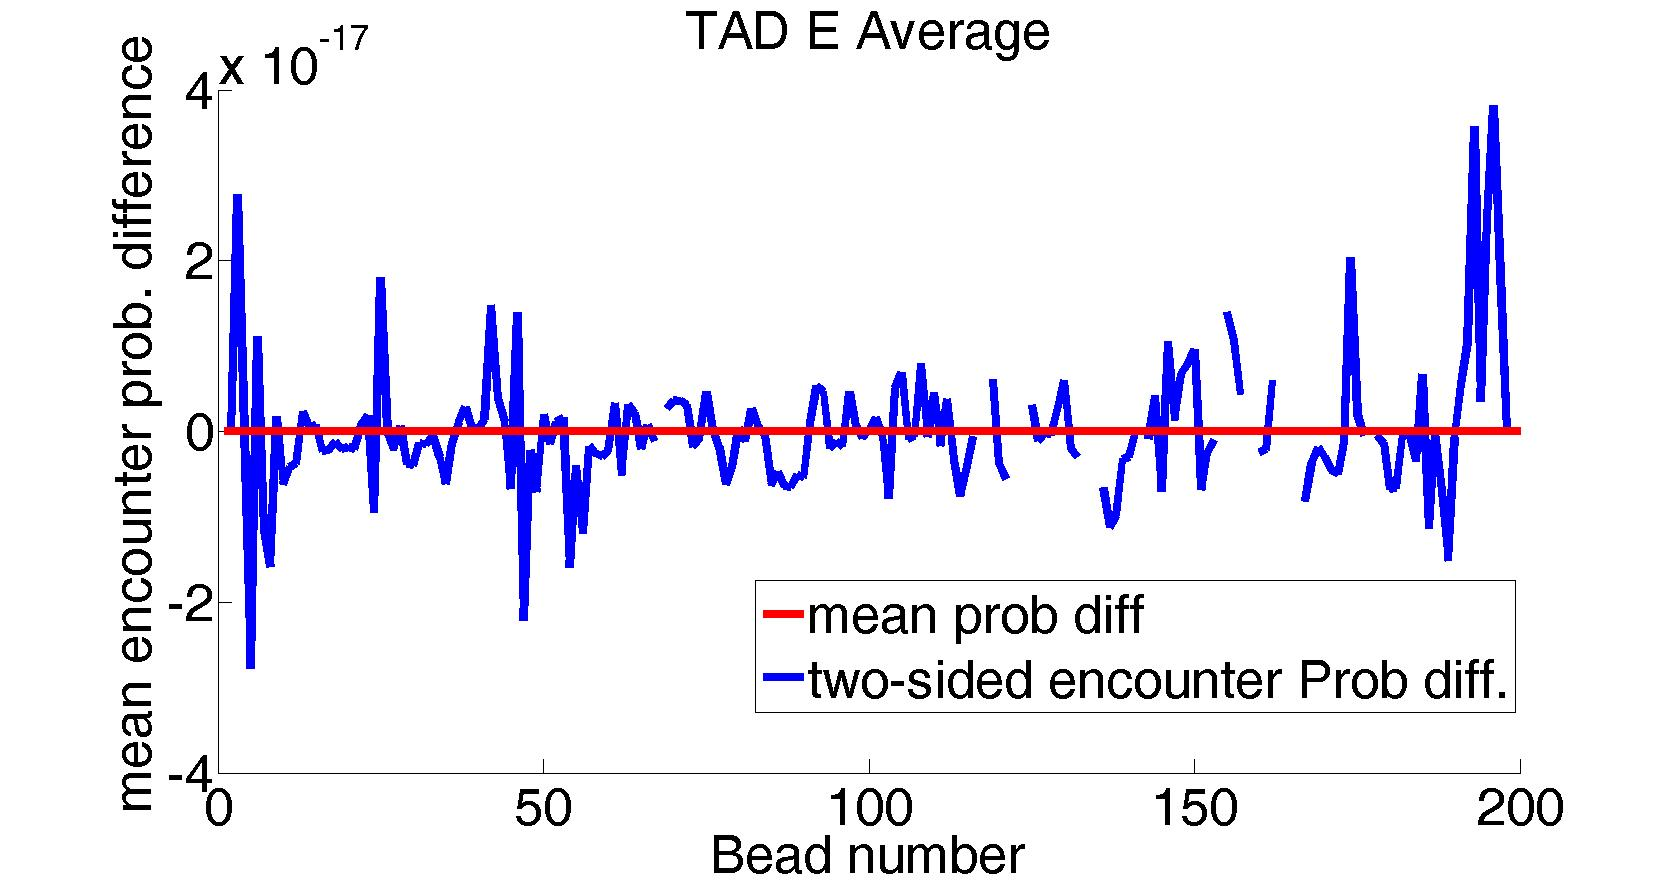
\includegraphics[scale=0.05]{symmetryOfTheEncounterProbabilityTADEAverage}
\end{figure}
\item TAD E has several strong specific interactions. TAD D has almost no specific interactions. Strong inter-TAD specific interactions
\end{itemize}

\begin{figure}[H]\label{TADDAndEencounterProb}
\centering
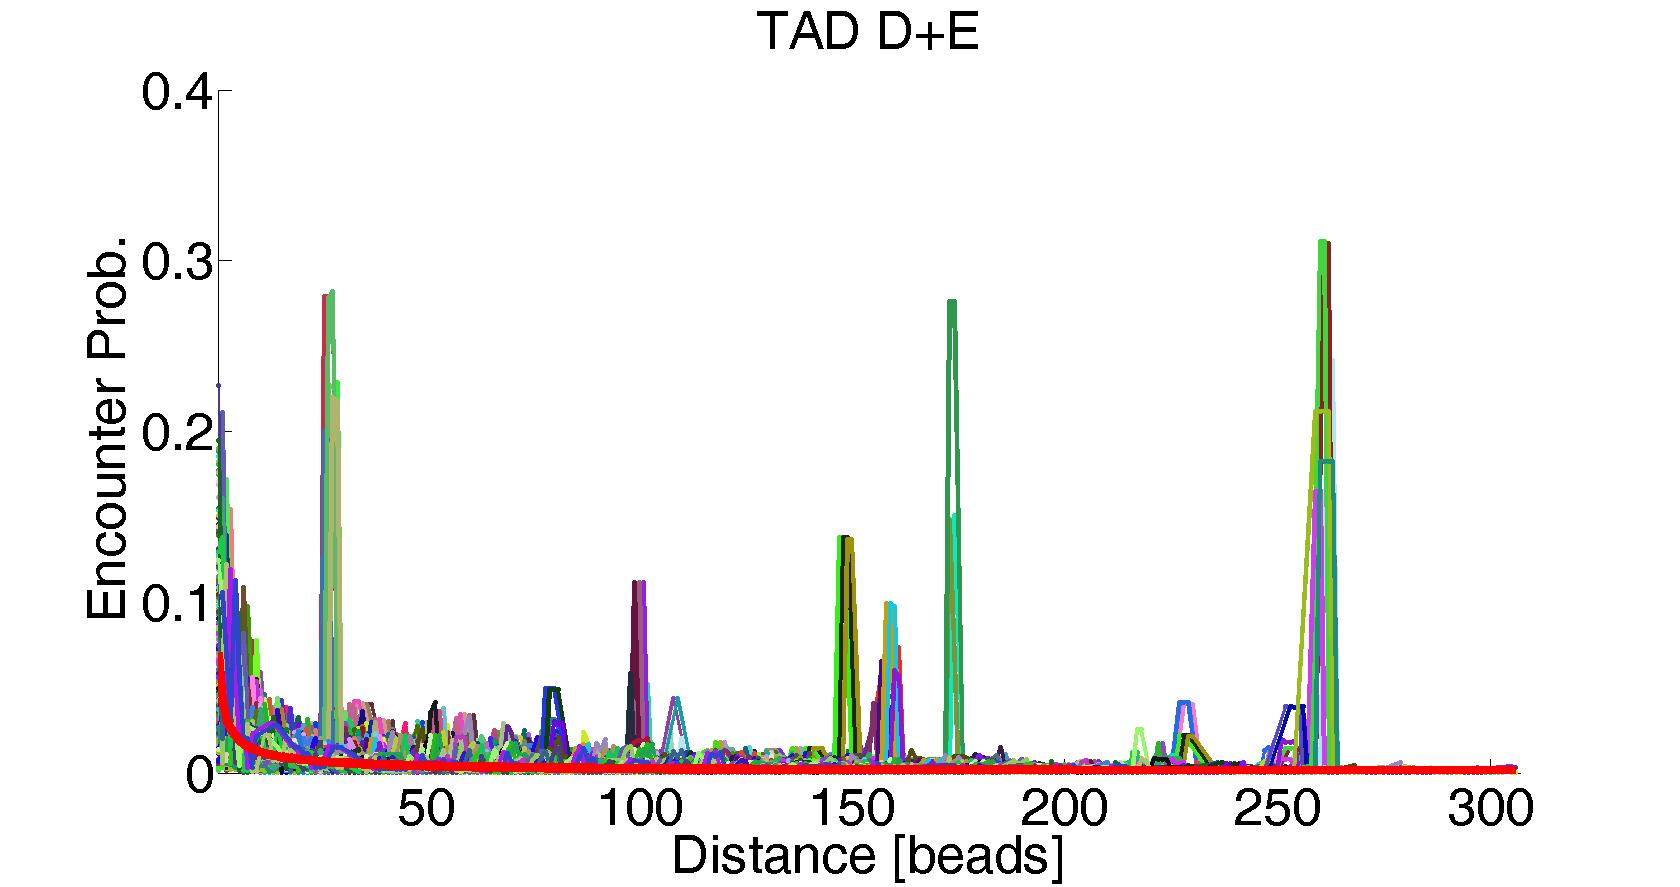
\includegraphics[scale=0.078]{encounterProbabilityTADDAndE}
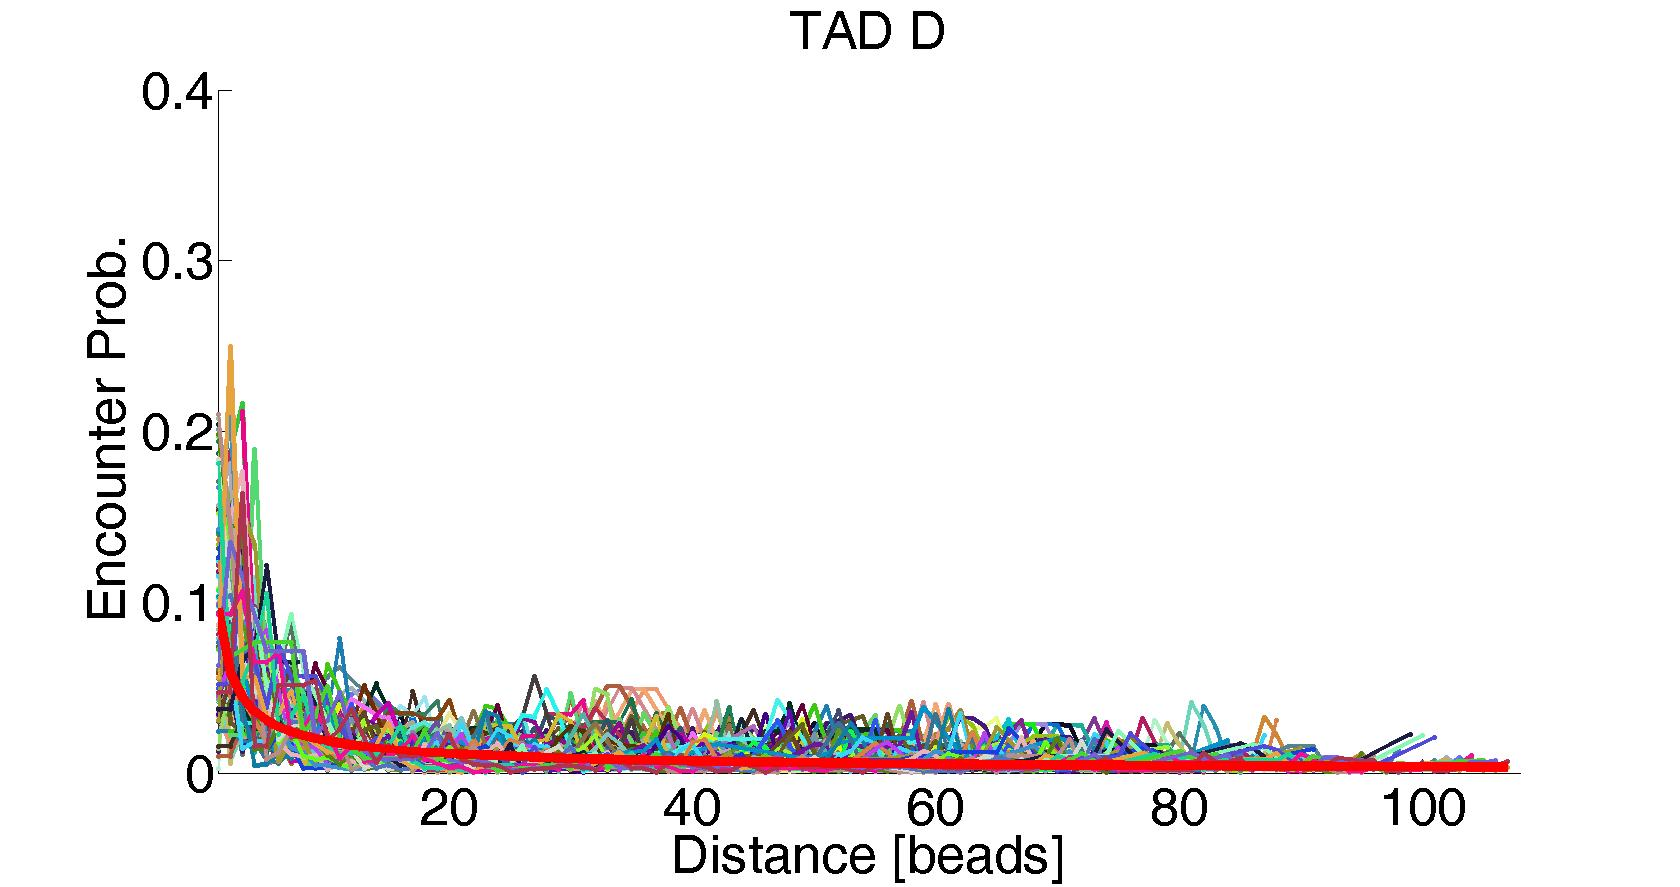
\includegraphics[scale=0.075]{encounterProbabilityTADD}
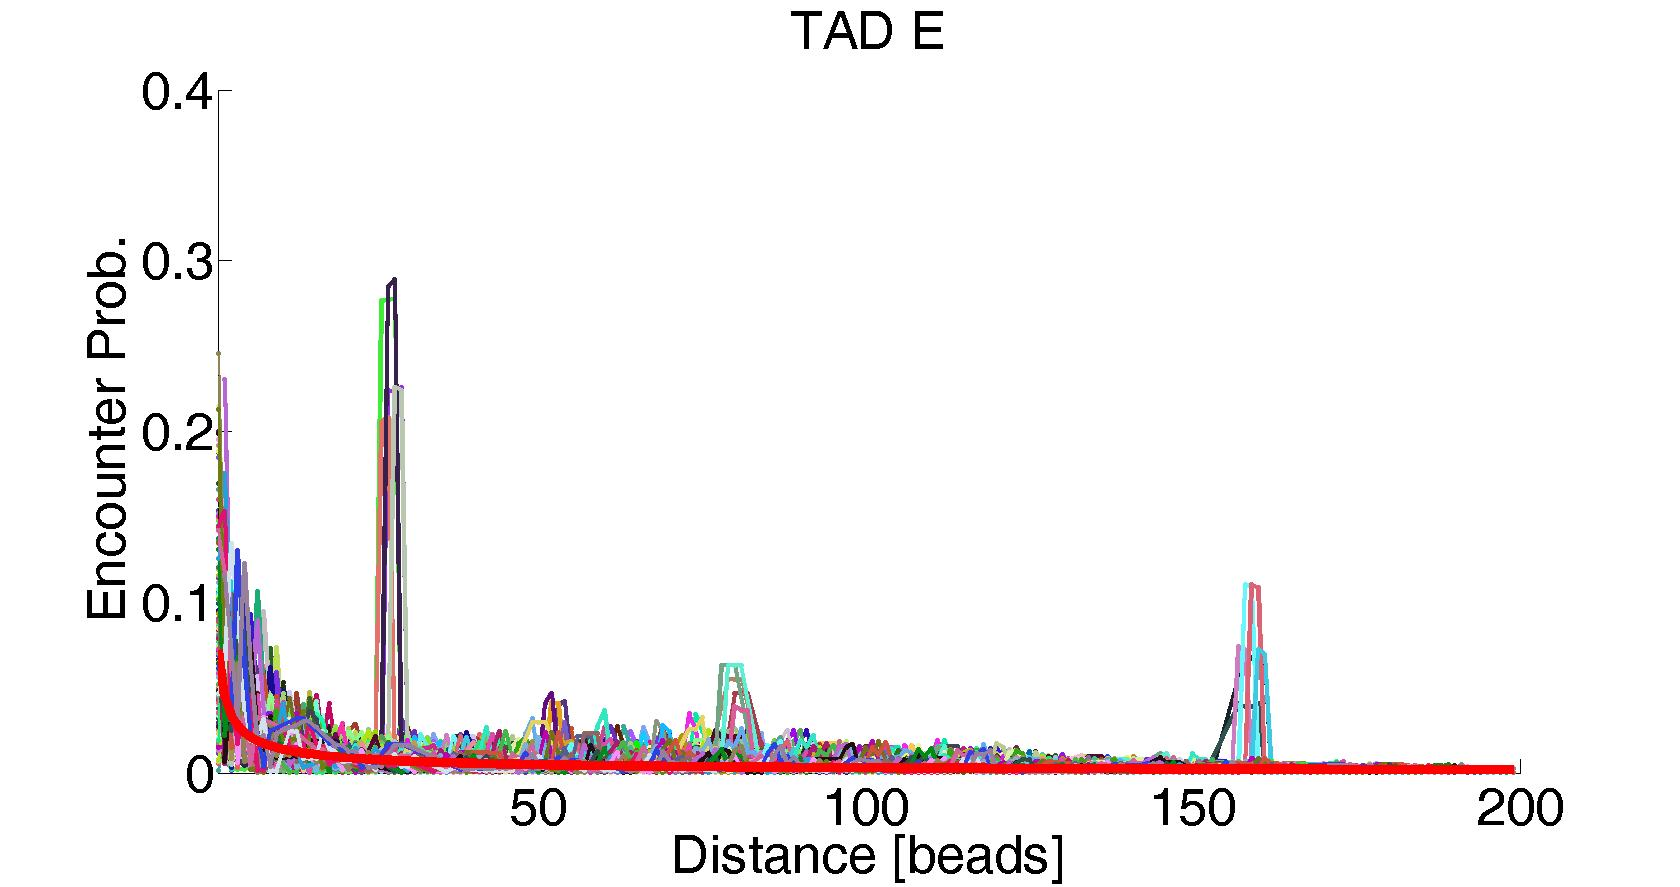
\includegraphics[scale=0.075]{encounterProbabilityTADE}
\end{figure}
\end{frame}

\subsection{Peaks of the encounter data}
\begin{frame}{Peaks of the encounter data}
\begin{itemize}
\item About half of the peaks in the encounter data result from specific interactions \textcolor{red}{between TADs}
\item The other half comes from specific internal interactions of \textcolor{green}{TAD E}.
\item To get an impression, a manual marking of the peaks shows 
\end{itemize}
\begin{table}[H]\label{nonNeighborBeadEncounterTable}
\begin{tabular}{l l l}
Bead numbers & Encountered beads & TAD\\
\hline
23-26   & 280-290 & \textcolor{red}{$D\leftrightarrow E$}\\
49-53   & 148-155 & \textcolor{red}{$D\leftrightarrow E$}\\
56-59   & 80-90   & $D\leftrightarrow D$\\
115-117 & 165-170 & \textcolor{green}{$E\leftrightarrow E$}\\
161-162 & 187 190 & \textcolor{green}{$E\leftrightarrow E$}\\
182-184 & 260-264 & \textcolor{green}{$E\leftrightarrow E$}\\
185-186 & 253-255 & \textcolor{green}{$E\leftrightarrow E$}\\
234-236 & 184-189 & \textcolor{green}{$E\leftrightarrow E$}\\
234-236 & 4-11    & \textcolor{red}{$E\leftrightarrow D$}\\
243     & 88      & \textcolor{red}{$E\leftrightarrow D$}\\
264     & 89-90   & \textcolor{red}{$E\leftrightarrow D$}\\
274-277 & 113-120 & \textcolor{green}{$E\leftrightarrow E$}
\end{tabular}
\end{table} 
\end{frame}

\subsection{The encounter probability}\label{subsection_theEncounterProbability}
\begin{frame}{The enconter probability}
For the case of TAD D, TAD E, and the two together, we estimate the bead encounter probability, $p$, and fit it with a function of the form 
\begin{equation*}
p_n(d)=\alpha d^{-\beta}
\end{equation*}
where, $d$ is the distance in bead units, $\alpha=\frac{1}{\sum_{j=1}^{d_{max}}j^{-\beta}}$ and $\beta$ is a parameter to be estimated.
We report the values of $\beta$ for each bead in each case
\begin{figure}[H]
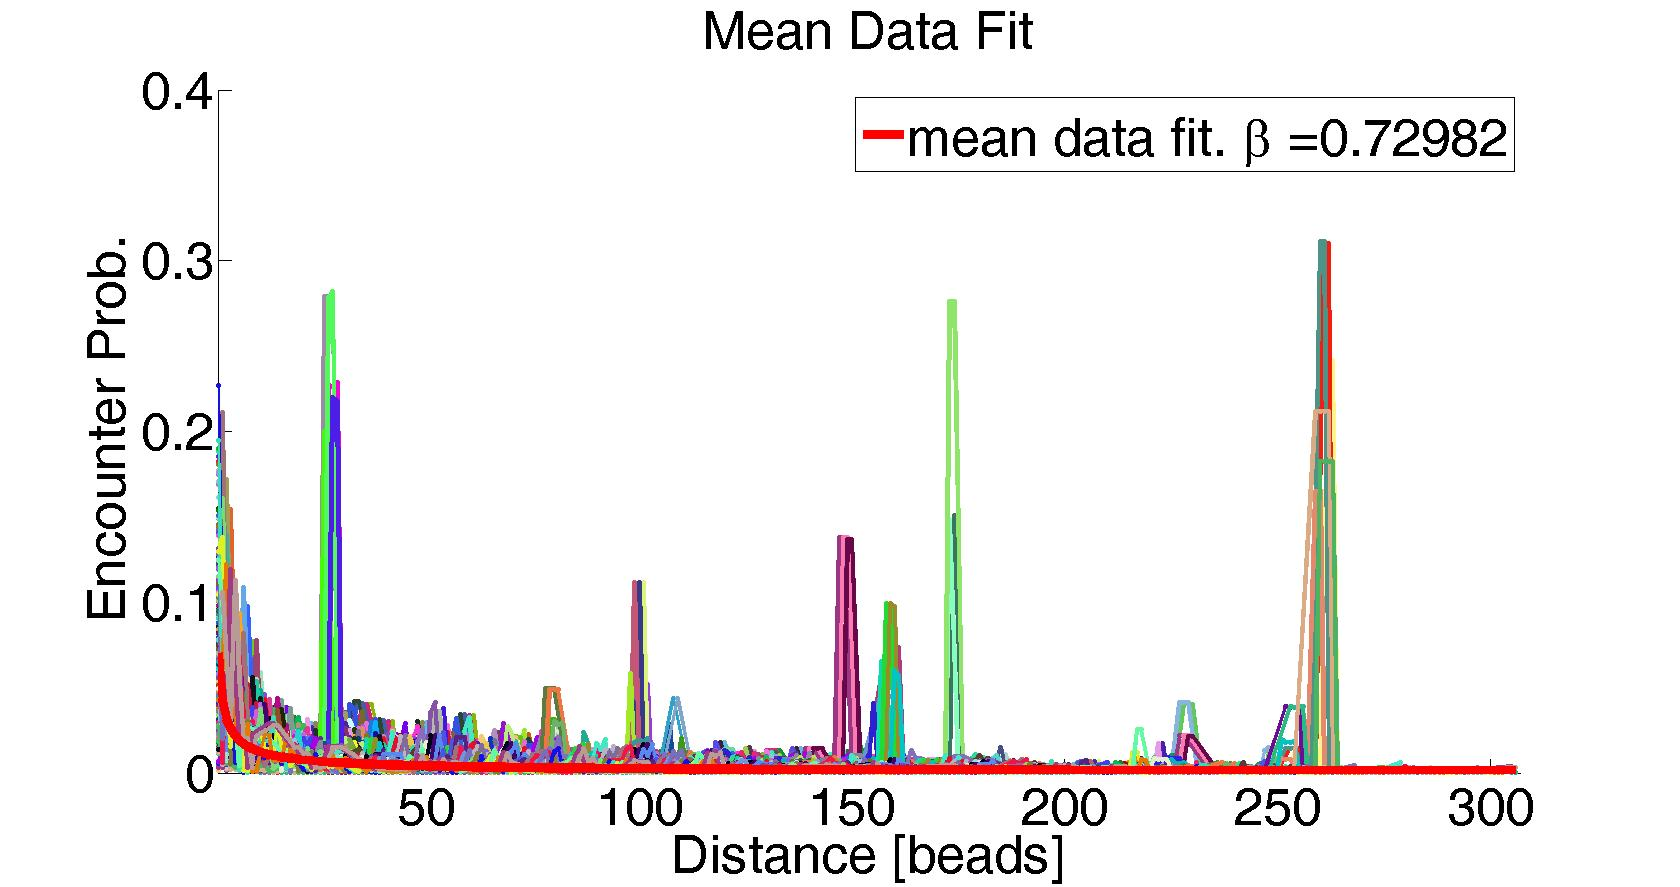
\includegraphics[scale=0.1]{meanDataFitTADDAndE}
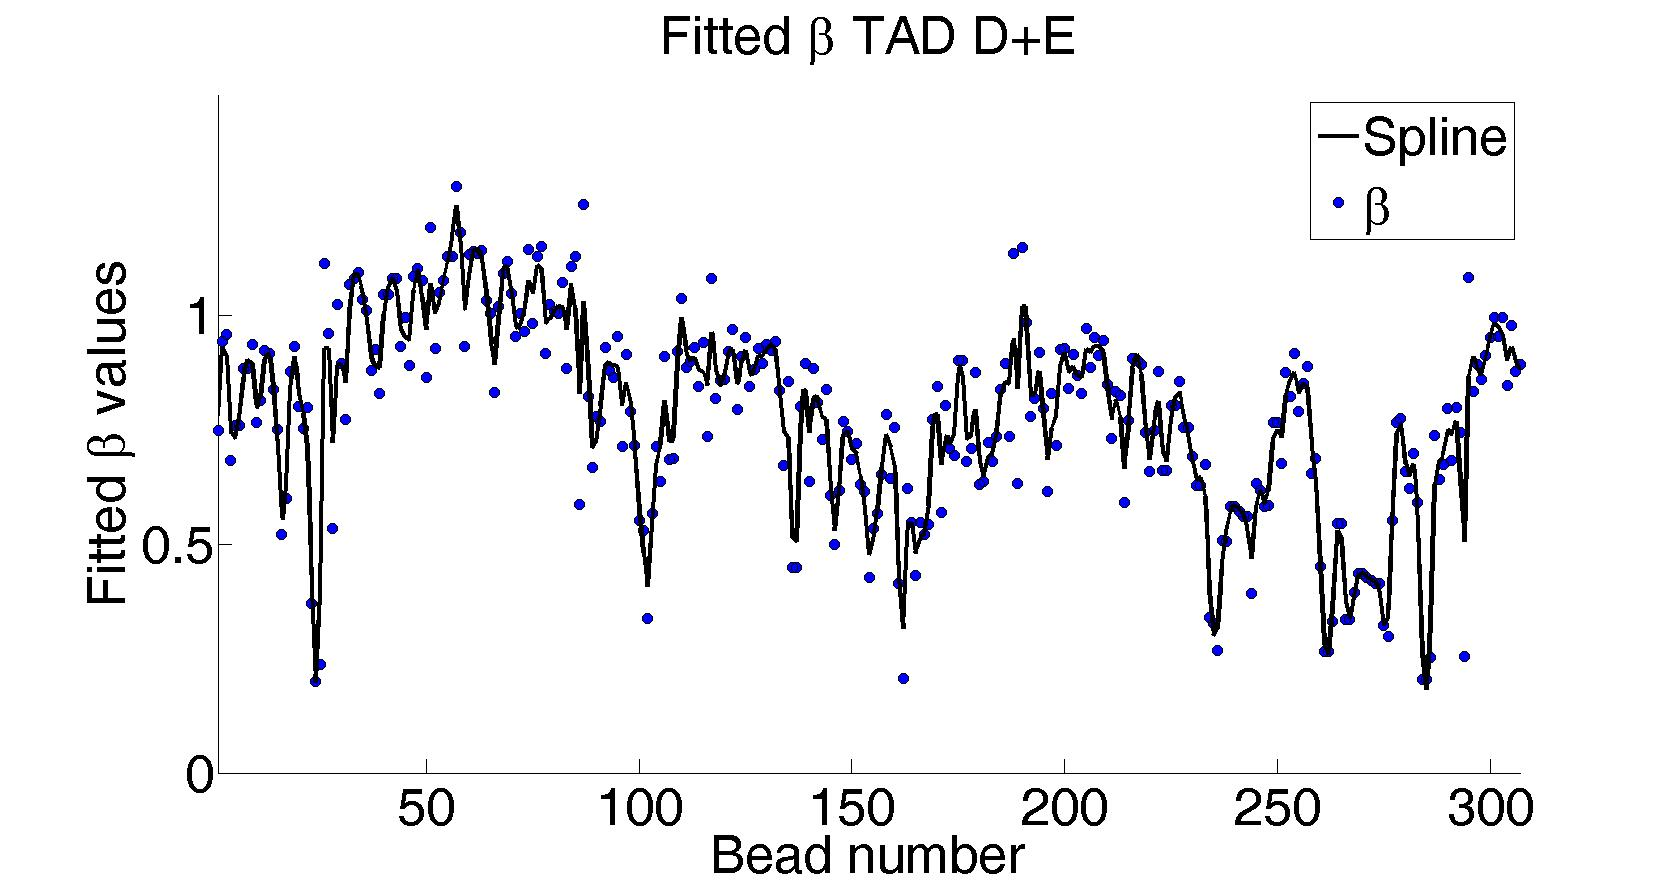
\includegraphics[scale=0.1]{fittedExpValuesWithSplineAverageTADDAndE}
\end{figure}
\end{frame}

\section{Theoretical model}\label{section_theoreticalModel}
\begin{frame}{Theoretical model}
\framesubtitle{The Rouse model}
We start with the classical and most simple model, the Rouse chain.
\begin{itemize}
\item A Rouse chain describes polymer dynamics as a stochastic motion of a collection of microscopic "beads" connected by harmonic springs
\item the 3D  motion of bead $n$ in the chain of $N$ beads 
\begin{equation*}
\frac{dR_n}{dt} = -\frac{3D}{b^2}(2R_n(t)-R_{n+1}(t)-R_{n-1}(t))+f_n(t)
\end{equation*}
\item $R_n$- the position of bead $n$\\
$b$- the standard deviation of the distance between adjacent beads\\
$D$- the diffusion constant\\
$f_n$- white Gaussian noise
\item From the theory, $Pr(\|R_n-R_m\|<\epsilon)\sim  |n-m|^{-1.5}$
\end{itemize}
\end{frame}

\section{Simulations}
%simulation section order:
% 1. normal Rouse 
% 2. normal rouse with peaks
% 3. 
\subsection{Simulations with a simple rouse chain}
\begin{frame}{Simulation with simple rouse chain}
\begin{itemize}
\item we first check whether a simple model can produce the TADs. 
\item we examine the results of simulating  chain of 64 beads
\end{itemize}

\end{frame}

\subsection{Loops corresponding to the peaks of the encounter data}
\begin{frame}{Loops corresponding to the peaks of the encounter data}

\end{frame}

\subsection{Dynamic loops model}
\begin{frame}{Dynamic Loop Model}
\begin{itemize}
\item some beads in the same TAD have affinity toward one another
\item affine beads located within a distance less than $\epsilon$ (the encounter distance) are connected
\item the rate of disconnection between beads is $k_{off}$
\end{itemize}
\end{frame}

\subsection{Dynamic loops model with beads' affinity}
\begin{frame}{Dynamic loops model with beads affinity}
\end{frame}

\subsection{Enlarging the encounter distance}
\begin{frame}{Enlarging the encounter distance}
\end{frame}

\subsection{3C experiment with stiff connectors}
\begin{frame}{3C experiment with stiff connectors}
Next, we simulate 64 bead chains with stiff connectors.\\
Stiff connectors are Rouse spring that stay fixed.\\
\end{frame}

\section{Future Perspectives}
\begin{frame}{Future perspective}
\begin{itemize}
\item A model with variable encounter distance
\item 
\end{itemize}
\end{frame}

\end{document}